\documentclass{minimal}
\usepackage{lmodern}
\usepackage{tikz}
\usetikzlibrary{arrows.meta,positioning,calc,fit}
\usepackage{xcolor}

\definecolor{ink}{HTML}{17202A}
\definecolor{muted}{HTML}{59636E}
\definecolor{paper}{HTML}{FAFBFC}
\definecolor{historyfill}{HTML}{E8F0F7}
\definecolor{statefill}{HTML}{DDF3EC}
\definecolor{transfill}{HTML}{E9E3F5}
\definecolor{closurefill}{HTML}{FCEBD7}
\definecolor{testblue}{HTML}{EAF2FA}
\definecolor{testgreen}{HTML}{E7F5EF}
\definecolor{testpurple}{HTML}{F0ECF8}
\definecolor{blue}{HTML}{2D6A9F}
\definecolor{green}{HTML}{278064}
\definecolor{purple}{HTML}{6B55A3}
\definecolor{orange}{HTML}{B66A20}

\pdfpagewidth=1000pt
\pdfpageheight=290pt
\setlength{\paperwidth}{1000pt}
\setlength{\paperheight}{290pt}
\setlength{\textwidth}{1000pt}
\setlength{\textheight}{290pt}
\setlength{\oddsidemargin}{-72pt}
\setlength{\topmargin}{-72pt}
\setlength{\headheight}{0pt}
\setlength{\headsep}{0pt}
\setlength{\footskip}{0pt}
\setlength{\parindent}{0pt}
\pagestyle{empty}

\begin{document}
\begin{tikzpicture}[
  x=1pt,y=1pt,
  font=\sffamily,
  line cap=round,
  line join=round,
  flow/.style={-{Latex[length=10pt,width=7pt]},draw=ink,line width=2.2pt},
  thinflow/.style={-{Latex[length=7pt,width=5pt]},draw=muted,line width=1.5pt},
  trainlink/.style={<->,>=Latex,draw=orange,densely dashed,line width=1.4pt},
  component/.style={rounded corners=8pt,draw=ink,line width=1.7pt,align=center},
  pill/.style={rounded corners=10pt,draw=purple,line width=1.3pt,fill=paper,
               minimum height=18pt,inner xsep=8pt,align=center},
  panel/.style={rounded corners=10pt,draw=ink!40,line width=1.2pt}
]
\useasboundingbox (0,0) rectangle (1000,290);
\fill[paper] (0,0) rectangle (1000,290);

% --- Evidence-layer header --------------------------------------------------
\node[anchor=west,text=ink,font=\sffamily\bfseries\fontsize{18}{21}\selectfont]
  at (25,280) {One TerraState checkpoint: inference path and matched evidence};
\node[anchor=east,text=muted,font=\sffamily\fontsize{14.4}{17}\selectfont]
  at (975,280) {Q1--Q3 core \quad+\quad optional post-training Q4};
\draw[ink!20,line width=1pt] (25,268) -- (975,268);

% --- Main TerraState pipeline ----------------------------------------------
% Cloud-masked history stack
\draw[rounded corners=5pt,fill=historyfill!55,draw=blue!55,line width=1.1pt]
  (32,159) rectangle (142,227);
\draw[rounded corners=5pt,fill=historyfill!75,draw=blue!70,line width=1.2pt]
  (26,165) rectangle (136,233);
\draw[rounded corners=5pt,fill=historyfill,draw=ink,line width=1.7pt]
  (20,171) rectangle (130,239);
\draw[blue!55,line width=3pt] (34,186) -- (52,204) -- (66,195) -- (81,217) -- (109,191);
\fill[paper,opacity=.9] (76,206) circle (14pt);
\fill[paper,opacity=.9] (92,212) circle (18pt);
\node[text=ink,font=\sffamily\bfseries\fontsize{13.5}{16}\selectfont,align=center]
  at (75,155) {cloud-masked history};

\node[component,fill=historyfill,minimum width=76pt,minimum height=52pt,
      font=\sffamily\bfseries\fontsize{17}{20}\selectfont]
  (q) at (191,205) {$q_{\theta,\rho}$};
\node[text=muted,font=\sffamily\fontsize{14.4}{17}\selectfont] at (191,245)
  {context/state inference};

\node[component,fill=statefill,minimum width=82pt,minimum height=58pt,
      font=\sffamily\bfseries\fontsize{18}{21}\selectfont]
  (zt) at (302,205) {$z_t$};
\node[text=green,font=\sffamily\bfseries\fontsize{14.4}{17}\selectfont]
  at (302,164) {spatial state};

\node[component,fill=transfill,minimum width=170pt,minimum height=70pt,
      font=\sffamily\bfseries\fontsize{18}{21}\selectfont]
  (trans) at (492,205) {shared $T_\psi$};
\node[text=muted,font=\sffamily\fontsize{14.4}{17}\selectfont]
  at (492,186) {weather-driven state advance};

\node[pill,font=\sffamily\fontsize{13.5}{16}\selectfont] (weather) at (400,253)
  {full24 weather};
\node[pill,font=\sffamily\fontsize{13.5}{16}\selectfont] (geo) at (505,253)
  {static $g$};
\node[pill,font=\sffamily\fontsize{13.5}{16}\selectfont] (elapsed) at (582,253)
  {horizon $h$};

\node[component,fill=statefill,minimum width=92pt,minimum height=58pt,
      font=\sffamily\bfseries\fontsize{18}{21}\selectfont]
  (zh) at (664,205) {$z_{t+h}$};
\node[text=green,font=\sffamily\bfseries\fontsize{14.4}{17}\selectfont]
  at (664,164) {advanced state};
\node[pill,draw=orange,text=orange,minimum width=118pt,
      font=\sffamily\fontsize{12.5}{15}\selectfont,align=center]
  (futuretarget) at (706,253) {frozen future-state target\\training only};

\node[component,fill=closurefill,minimum width=124pt,minimum height=70pt,
      font=\sffamily\bfseries\fontsize{15}{18}\selectfont]
  (closure) at (810,205) {closure $O_\omega$\\$b_h+O_\omega(z_{t+h})$};

\node[component,fill=paper,minimum width=92pt,minimum height=70pt,
      font=\sffamily\bfseries\fontsize{17}{20}\selectfont]
  (pred) at (939,205) {prediction\\$\widehat y_{t+h}$};
\node[pill,draw=blue,text=blue,font=\sffamily\bfseries\fontsize{13.5}{16}\selectfont]
  at (939,155) {Q1 skill};

\draw[flow] (130,205) -- (q.west);
\draw[flow] (q.east) -- (zt.west);
\draw[flow] (zt.east) -- (trans.west);
\draw[flow] (trans.east) -- (zh.west);
\draw[flow] (zh.east) -- (closure.west);
\draw[flow] (closure.east) -- (pred.west);
\draw[thinflow,draw=blue]
  (q.south) -- ($(q.south)+(0,-28pt)$) -- node[above,text=blue,
  font=\sffamily\fontsize{13.5}{16}\selectfont] {context-only prior $b_h$}
  ($(closure.south)+(0,-28pt)$) -- (closure.south);
\draw[thinflow] (weather.south) -- ($(trans.north)+(-55pt,0)$);
\draw[thinflow] (geo.south) -- (trans.north);
\draw[thinflow] (elapsed.south) -- ($(trans.north)+(55pt,0)$);
\draw[trainlink] (futuretarget.south) -- (zh.north);

% --- Test panels ------------------------------------------------------------
\node[panel,fill=testblue,minimum width=286pt,minimum height=130pt,anchor=south west]
  (q2p) at (25,10) {};
\node[anchor=north west,text=blue,font=\sffamily\bfseries\fontsize{17}{20}\selectfont]
  at (43,136) {Q2 \; Is the state load-bearing?};
\node[component,fill=paper,draw=blue,minimum width=92pt,minimum height=38pt,
      font=\sffamily\fontsize{14.4}{17}\selectfont] (q2full) at (87,80) {full};
\node[component,fill=paper,draw=blue,minimum width=92pt,minimum height=38pt,
      font=\sffamily\fontsize{14.4}{17}\selectfont] (q2cut) at (200,101) {closure cut $s=0$};
\node[component,fill=paper,draw=blue,minimum width=92pt,minimum height=38pt,
      font=\sffamily\fontsize{14.4}{17}\selectfont] (q2id) at (200,59) {$T\to I$};
\draw[thinflow,draw=blue] (q2full.east) -- (q2cut.west);
\draw[thinflow,draw=blue] (q2full.east) -- (q2id.west);
\node[anchor=south,text=muted,font=\sffamily\fontsize{14.4}{17}\selectfont,align=center]
  at (168,14) {paired skill loss + output change};

\node[panel,fill=testgreen,minimum width=300pt,minimum height=130pt,anchor=south west]
  (q3p) at (337,10) {};
\node[anchor=north west,text=green,font=\sffamily\bfseries\fontsize{17}{20}\selectfont]
  at (355,136) {Q3 \; Does weather drive the state?};
\node[component,fill=paper,draw=green,minimum width=88pt,minimum height=36pt,
      font=\sffamily\fontsize{14.4}{17}\selectfont] (matched) at (389,82) {matched};
\node[component,fill=paper,draw=green,minimum width=88pt,minimum height=36pt,
      font=\sffamily\fontsize{14.4}{17}\selectfont] (mean) at (493,103) {norm. mean};
\node[component,fill=paper,draw=green,minimum width=104pt,minimum height=36pt,
      font=\sffamily\fontsize{14.4}{17}\selectfont] (donor) at (555,60) {season/geo donor};
\draw[thinflow,draw=green] (matched.east) -- (mean.west);
\draw[thinflow,draw=green] (matched.east) -- (donor.west);
\node[anchor=south,text=muted,font=\sffamily\fontsize{14.4}{17}\selectfont,align=center]
  at (487,14) {other inputs fixed; state + output change};

\node[panel,fill=testpurple,minimum width=312pt,minimum height=130pt,anchor=south west]
  (q4p) at (663,10) {};
\node[anchor=north west,text=purple,font=\sffamily\bfseries\fontsize{16}{19}\selectfont]
  at (681,136) {Q4 \; Optional post-training composition};
\node[component,fill=paper,draw=purple,minimum width=92pt,minimum height=38pt,
      font=\sffamily\fontsize{14.4}{17}\selectfont] (direct) at (730,92) {direct\\$T(h_1{+}h_2)$};
\node[component,fill=paper,draw=purple,minimum width=112pt,minimum height=38pt,
      font=\sffamily\fontsize{14.4}{17}\selectfont] (composed) at (730,52) {composed\\$T(h_2)\circ T(h_1)$};
\node[component,fill=paper,draw=purple,minimum width=112pt,minimum height=42pt,
      font=\sffamily\fontsize{14.4}{17}\selectfont] (guard) at (906,72) {same endpoint\\accuracy guard};
\draw[thinflow,draw=purple] (direct.east) -- (guard.west);
\draw[thinflow,draw=purple] (composed.east) -- (guard.west);
\node[anchor=south,text=muted,font=\sffamily\fontsize{11.5}{13}\selectfont,align=center]
  at (819,14) {same $T_\psi$; no training loss; endpoint/non-collapse guards};

\end{tikzpicture}
\end{document}
